\chapter{Introduction}
\section{What this course will teach}
This workshop will introduce the student to Python coding, electronics, and project
design. We will be building several projects ranging from simple (less components and
simpler code) to more complex (more components or more complicated code). These projects
are based on the ESP32-C3 microcontroller (specifically the development board produced by
\href{https://www.seeedstudio.com/Seeed-XIAO-ESP32C3-p-5431.html}{Seeed Studio}) which is
running MicroPython and they depend on some other electronics components such as LEDs,
buttons, and more.

Students are encouraged to make use of the written instructions and diagrams and to
explore and play with the components for themselves to see how they work and what
they do. There are many online resources as well for learning.

\section{Project Kit Contents}
\begin{figure}[H]
\centering
    \includegraphics[width=\linewidth]{common/case_and_parts.png}
    \caption{This image shows all of the contents of the project kit and labels what each one is}
\end{figure}

\section{Working with the microcontroller}
\subsection{Installing the driver}
Connecting the microcontroller to your computer may require the installation of a
USB driver. If so, download the driver for your OS from this page and install as instructed:
\url{https://ftdichip.com/drivers/vcp-drivers/}. Once installed successfully, unplug and replug
the USB cable into the microcontroller and then press the small reset button on the
microcontroller board labeled "R" (for reset).

\subsection{Pinout Reference} \label{pinout}
On any integrated circuit, that is a chip that contains electronic logic, a pinout is
a diagram and description of what each of the pins of that circuit are used for. This is
a very useful document for any electronics engineer to have handy and to reference. The
pinout diagram for the microcontroller that we are using as part of this workshop is
replicated below:
\begin{figure}[H]
\centering
    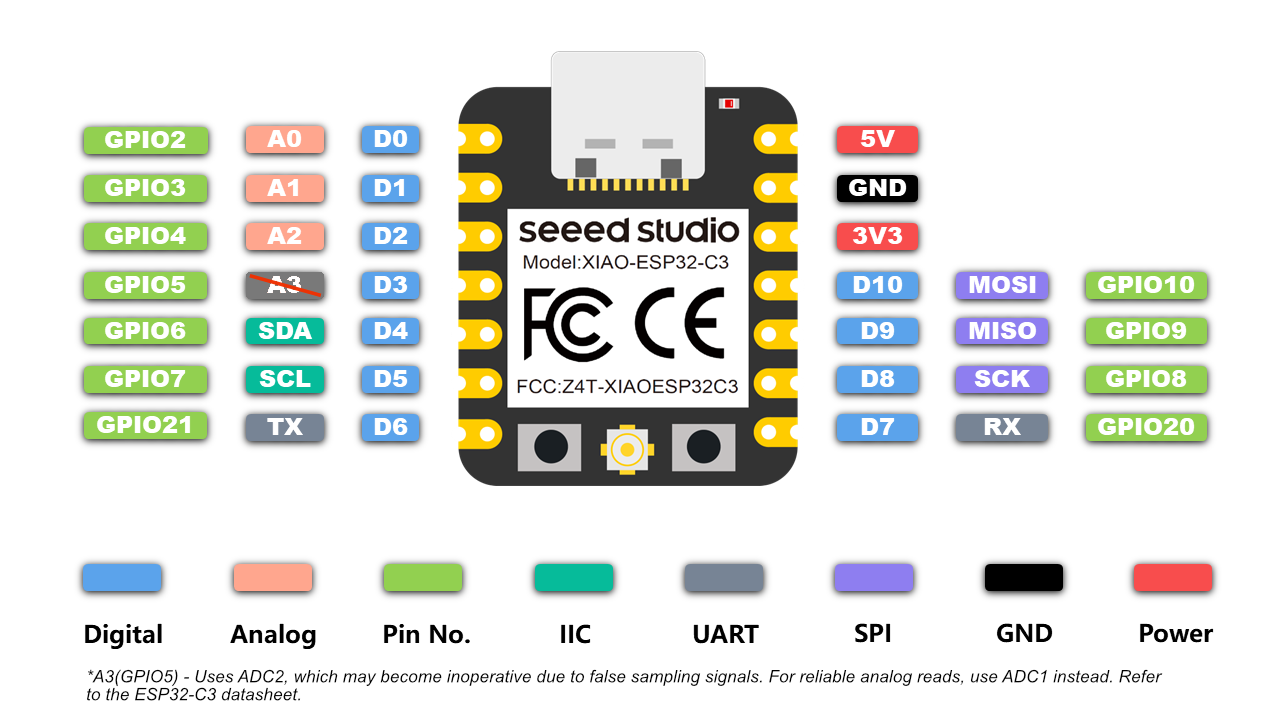
\includegraphics[width=.6\linewidth]{common/esp32c3_pinout.png}
    \caption{A simplified pinout of the Seeed Studio ESP32-C3 development board}
\end{figure}

In this diagram, you'll notice several things:
\begin{itemize}
    \item An image of the microcontroller board in the center
    \item A label for each pin indicating its function
\end{itemize}

In the code throughout this guide, you will see references to pin numbers like \textbf{Pin(5)}.
Wherever you see this, it means that the code is expecting a connection to, in this example, the
4th pin down on the left. If you find that your code is not working as expected, double check the
pin numbers in the code vs. the placement of your wires.